\chapter{Detection of cells \status{in progress}}
	\label{chap:cell_detection}
	
	\section{Cell detection overview \statusfirstdraft}
	
	In order to track cells across frames we need to first be able to identify the cells within the images. As described in \cref{sec:relatedworkdetection}, there is a broad range of automatic methods for cell detection and segmentation.
	
	The requirements for detecting cells in our application are:
		
	\begin{enumerate}
	\item Accurate detection in sometimes noisy images. The detector should be able to robustly identify cells in datasets that include noise, motion artefacts (induced by the camera and the moving tissue) and variable lens focus. The detector does not need to detect cells that are out of focus, but should reliable detect those are in focus. Out of focus frames are dealt with in the tracking module.
	
	\item There is no need for accurate segmentation. We are primarily interested in the accurate tracking of cells, and analysis of the cells appearance is of secondary interest. For the purpose of tracking, it is sufficient to be able to reliable localize cells, and extract some features that identify these cells.
	
	\item The algorithm should adapt well to different microscopy modalities. The studied datasets are obtained from various organs within the body of mice that have distinct textures. The detector should be able to detect cells in any of these datasets with minimal  manual adjustments.
	\end{enumerate}
	
	Much of the previous work described in \cref{sec:relatedworkdetection} was focused on accurate segmentations of cells. Many of the described methods would return very good segmentations, but they would fail when presented with a very noisy dataset of varying contrast, or need major manual tuning of parameters when presented with a new dataset with a different kind of cells.
	
	For the purpose of our application we have chosen the cell detector presented in \cite{arteta12}, because it conforms to all three requirements. The machine learning method is able to handle noisy datasets, and the model can easily be retrained when a new, previously unseen, type of images needs to be analysed. The method does not focus on accurate segmentation of cells, but on the robust localization. The major drawback of this method was performance. The authors reported run-times of 30 seconds to detect cells on 400-by-400 pixel images on an i7 CPU. This slow performance would make it unusable for tracking large image sequences. However, we were able to optimize the MATLAB code for feature computation so that the detection process takes only a fraction of the original run-time.
	
	The detection process runs in three steps. First, robust candidate regions are extracted from an image. The method uses an efficient MSER region detector \addref{} to find a large number of candidate regions. Second, each of these regions is assigned a value which is produced by a classifier, which indicates the appropriateness score that this this region is a cell. Finally, the non-overlapping subset of these candidate regions with high similarity to the annotated cells in the training data is selected via dynamic programming.
	
	The detector can be trained on a small number of training images, where each cell is  annotated with a single dot. 

	The code used in our method is based on the original code from \cite{arteta12}. Some of our modifications, especially in the feature computations, allow the detector to run significantly faster. Additional work was required to combine the cell detector with the tracking module described in \cref{chap:tracking}.
	
	The remained of this chapter is divided as follows. In \cref{sec:detector_extremal} we describe how the candidate regions are obtained. \Cref{sec:detector_inference} shows the inference procedures that selects the optimal subsets of candidate regions. In \cref{sec:detector_classifier} we formulate the learning method and in we describe the choice of features in \cref{sec:detector_feature}. Finally, in \cref{sec:detector_changes} we briefly outline the main changes that improved the performance of the original algorithm.
	
	\section{Detection of candidate regions \statusnew}
	\label{sec:detector_extremal}
	
	what is their work in the detector: they are candidates cells, that are then evaluated as cell/nocell	
	
	what are extremal regions
	
	the nestedness porperty
			
	what ia a maximally stable region
	
	and that they are obtained from the MSER featre detector
	
	why are they good: fast, robust to contrast and to what else
		
	exapmle of these regions in cell images
	
	\section{Inference under the non-overlap constraint \statusnew}
	\label{sec:detector_inference}
	
	the value from the classifier score. 
	
	that we pick a subset such that we maximise the sum of score of the picked regions, while preserving the non-overlap property.
	
	Specifically, The formulation of the model
	
	how the nestedness property helps
	
	why is that ok: the datasets don't exhibit such behavior. much more training data would be required, which means more annotations.
	
	\section{Learning the classifier}
	\label{sec:detector_classifier}
	
	gives a score 
	
	using dot annotation
	
	what are the inputs, that we defined some features for each regions
	
	that we use a linear classifier to scroe each region, understand and review the goal of learning
	
	why wec hose structured learing.
	
	structural svm, why?
	
	the loss function
	
	the convex objective
	
	leave the details of the cutting plane to read by the viewer.
		
	\section{Feature selection \status{new}}
	\label{sec:detector_feature}
	
	The effictiveness of the machine learning method to detect cells depends on the quality of features. Good features have a lot of discriminative power between cells and non cells. The used approach classifies extremal regions as cell/non-cell. The regions are extracted using the MSER detector. Then each region is processed and features are extracted from it. We have evaluated several combinations of these features:
	
	\begin{enumerate}
	    \item the area A of the region represented by a 10-dimensional binary vector with the entry $\lceil log A \rceil $ set to 1.
		\item 10-dimensional histogram of intensities within the region
	    \item the position of the descriptor in the image in terms of x-y coordinates of a centroid fitted to the descriptor.
	    \item two 6-dimensional histograms of differences in intensities between the region border and a dilation of it for two different dilation radii
	    \item a shape descriptor represented by a 60-dimensioal histogram of the distribution of the boundary of the region on a size-normalized polar coordinate system
	    \item The orientation of the descriptor after attempting to normalize its orientation
	    \item The proportion of edge-pixels in the region.
	\end{enumerate}
	
	Each of these features has different discriminative power, and takes some time to compute. The application of the cell detector requires that images are processed within a time limit. For this reason, we have trained and tested the algorithm with all the $2^7 - 1$ possible combinations of these features.
	
	We have also developed a function that helps select the most appropriate set of features given specific constraints, for example a maximum computation time, minimal precisiona and recall values, etc. A graph generated by the function is shown in figure \ref{fig:bestFeatureSelector}.
	
	\begin{figure}
		  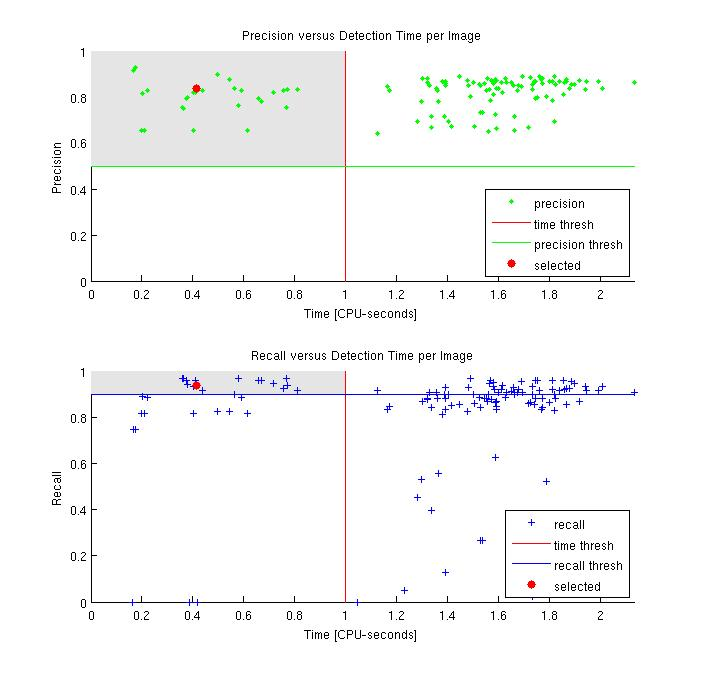
\includegraphics[width=\textwidth]{images/best_features}
		\caption{The plots helps the user to select the most appropriate feature, given a combination of computation time per image, mean precision and recall. This example, which was obtained by selecting only within feature sets that compute in less than 1 CPU-second, have at least 0.5 precision and 0.9 recall have resultsed in a feature set containing features 1, 3 and 4. Most importance was given to precision followed by computation time and recall. The selected feature set computes in 0.414 cpu-seconds (Intel(R) Core(TM) i7-2600 CPU @ 3.40GHz) per image, with mean precision of 0.836 and mean recall of 0.9363.}
	    \label{fig:bestFeatureSelector}
	\end{figure}
	
	\section{Speeding up the algorithm \status{new}}
	\label{sec:detector_changes}
		\todo[inline]{review this section}
		The main drawback of the algorithm presented by Arteta \cite{arteta12} is the poor performance. The original algorithm took about 30 seconds to detect cells in a 400x400 image. Because we will be processing hours of microscopy video it was important to reduce the detection time as much as possible.  The major performance improvements where achieved by addressing three things.
		
		The algorithms needs to extract a set of feature on every single detecetd MSER. First, we have first fine-tuned the MSER detector to detect less cells, more robustly.
		
		Second, we have identified features that are slow to compute and improved their algorithmic behaviour. One such feature is the Contour Points Distribution Histogram implemented in \textit{cpdh.m}. The function was performing excessive calls to slow functions to extract region characteristics, and was rewritten to call these function less often, without affecting its value.
		
		Second, several MATLAB builtin function were modified to remove excessive parameter checking, which in several cases represented an overhead of over $30\%$. These parameter checks are welcome when developing the algorithm, but once the algorithm is complete, several of these checks can be safely removed. \rewrite{Not sure I can write this, since the matlab code is copyrighted}
		
		These opimizations resulted in a significant performance boost. Instead of 30 seconds, the algorithm can now detect cells on the same images in about \todo{Measure the number of seconds it takes to process one of these 400x400 images}.
		
	